%%%%%%%%%%%%%%%%%%%%%%%%%%%%%%%%%%%%%%%%%
% Trace Analysis and Monitoring
%
% $Date$
% $Rev$:
% $Author$

\chapter{\KiekerTraceAnalysis{} Tool}\label{chap:aspectJ}

\KiekerTraceAnalysis{} implements the special feature of \Kieker{} allowing to %
monitor, analyze, and visualize (distributed) traces of method executions and %
corresponding timing information. For this purpose, it includes monitoring probes employing %
AspectJ~\cite{AspectJ-WebSite}, Java~EE Servlet~\cite{JavaServletTechnology-WebSite}, %
Spring~\cite{Spring-WebSite}, and Apache~CXF~\cite{CXF-WebSite} technology. %
Moreover, it allows to reconstruct and visualize architectural models of the %
monitored systems, e.g., as sequence and dependency diagrams. %

Section~\ref{chap:example} already introduced parts of the monitoring record %
type \class{OperationExecutionRecord}. \KiekerTraceAnalysis{} uses this record %
type to represent monitored executions and associated trace and session information. %
Figure~\ref{fig:OperationExecutionRecordClassDiagramComplete} shows a class diagram %
with all attributes of the record type \class{OperationExecutionRecord}. %
The attributes \method{className}, \method{operationName}, %
\method{tin}, and \method{tout} have been introduced before. %
The attributes \method{traceId} and \method{sessionId} are used to store %
trace and session information; \method{eoi} and \method{ess} contain control-flow %
information needed to reconstruct traces from monitoring data. %
For details on this, please refer to our technical %
report~\cite{vanHoornRohrHasselbringWallerEhlersFreyKieselhorst2009TRContinuousMonitoringOfSoftwareServicesDesignAndApplicationOfTheKiekerFramework}.

\begin{figure}[hb]\centering
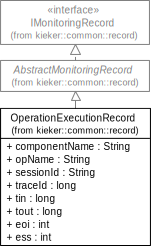
\includegraphics[scale=0.8]{images/kieker_OperationExecutionRecord-complete-modified}%
\caption{The class diagram of the operation execution record}
\label{fig:OperationExecutionRecordClassDiagramComplete}
\end{figure}

\enlargethispage{1cm}

\noindent Section~\ref{sec:traceMonitoring} describes how to instrument Java %
applications for monitoring trace information. %
It presents the technology-specific probes provided by \Kieker{} for this %
purpose---with a focus on AspectJ. %
Additional technology-specific probes can be implemented based on the existing %
probes. %
Section~\ref{sec:traceAnalysisTool} presents the %
tool which can be used to analyze and visualize the recorded trace %
data.  Examples for the available analysis and visualization outputs %
provided by \KiekerTraceAnalysis{} are presented in %
Section~\ref{sec:traceAnalysisExamples}.

\section{Monitoring Trace Information}\label{sec:traceMonitoring}

The following Sections describe how to use the monitoring probes based on %
AspectJ (Section~\ref{sec:traceAnalysis:instr:AspectJ}), %
the Java Servlet~API (Section~\ref{sec:traceAnalysis:instr:servlet}), %
the Spring Framework (Section~\ref{sec:traceAnalysis:instr:spring}), and %
Apache~CXF (Section~\ref{sec:traceAnalysis:instr:cxf}) provided %
by \Kieker{}. %

\subsection{AspectJ-Based Instrumentation}\label{sec:traceAnalysis:instr:AspectJ}

AspectJ~\cite{AspectJ-WebSite} allows to weave code into the byte code of %
Java applications and libraries without requiring manual modifications of the %
source code. %
\Kieker{} includes the AspectJ-based monitoring probes %
\class{OperationExecutionAspectAnnotation}, %
\class{OperationExecutionAspectAnnotationServlet}, %
\class{OperationExecutionAspectFull}, and %
\class{OperationExecutionAspectFullServlet} %
which can be woven into Java applications at compile time and load time. %
These probes monitor method executions and corresponding %
trace and timing information. The probes with the postfix \class{Servlet} %
additionally store a session identifier within the \class{OperationExecutionRecord}. %
When the probes with name element \class{Annotation} are used, %
methods to be monitored must be annotated by the \Kieker{} %
annotation \class{@OperationExecutionMonitoringProbe}. %
This section demonstrates how to use the AspectJ-based probes to monitor %
traces based on the Bookstore application from Chapter~\ref{chap:example}. %

\enlargethispage{1.0cm}

\NOTIFYBOX{The Java sources of the example presented in %
this section, as well as a pre-compiled binary, can be found in the %
\file{\aspectJBookstoreApplicationDirDistro{}/} directory of the %
binary release.}

% \

% This chapter will show in Section~\ref{sec:aspectJ:annotation} how
% to use AspectJ to mark methods to be monitored with a simple annotation
% in order to avoid the manual monitoring as seen in Chapter~\ref{chap:example}
% and \ref{chap:componentsMonitoring}. Once the methods are marked, the AspectJ-Weaver-Agent
% will surround the calls with the necessary code during runtime, similar
% to the manually inserted instrumentation code used in Section~\ref{sec:example:monitoring}.
% An alternative solution will be shown as well in Section~\ref{sec:aspectJ:fullweaving}, %
% where the methods to be instrumented are specified using an external configuration file %
% without requiring source code modifications. Both solutions
% can be used to reconstruct architectural views and to perform trace
% analyses. The result of both will be diagrams similar to sFigure~\ref{fig:bookstore:classAndSequenceDiagrams}.

% The idea of weaving the monitoring-code into the ``plain'' code
% during compile-time seems to suggest itself, but
% in this chapter it
% is only shown how to perform the so called load-time-weaving - the
% weaving during runtime.%, which is more flexible than the compile-time-weaving.

\begin{figure}[H]
\begin{graybox}
\dirtree{%
.1 \DirInDirTree{examples/}. %\DTcomment{The root directory of the project}.
.2 \DirInDirTree{userguide/}.
.3 \DirInDirTree{ch5--trace-monitoring-aspectj/}.
.4 \DirInDirTree{build/}\DTcomment{Directory for the Java class files}.
.5 \DirInDirTree{META-INF/}.
.4 \DirInDirTree{META-INF/} \DTcomment{Directory for the configuration files}.
.5 \newFileDirInDirTree{\aopConfigFile}.
.5 \kiekerMonitoringProperties{}.
.4 \DirInDirTree{lib/} \DTcomment{Directory for the needed libraries}.
.5 \newFileDirInDirTree{\mainJarWeaver}.
.4 \DirInDirTree{src/}\DTcomment{Directory for the source code files}.
.5 \DirInDirTree{bookstoreTracing/}.
.6 Bookstore.java.
.6 BookstoreStarter.java.
.6 Catalog.java.
.6 CRM.java.
}
\end{graybox}

\caption{The new directory structure of the Bookstore application}
\label{fig:bookstoreAOP:dirStructure}
\end{figure}

Figure~\ref{fig:bookstoreAOP:dirStructure} shows the directory used by the example of this section. %
The jar-file \file{\mainJarWeaver} already includes the \textit{AspectJ weaver}, %
which is registered with the JVM and weaves the monitoring instrumentation into %
the Java classes. It will be configured based on the configuration file %
\file{\file{\aopConfigFile}}, for which a working sample file is provided in the %
example's \dir{META-INF/} directory. Instead of registering the \file{\mainJarWeaver} %
as an agent to the JVM, the \file{\aspectJWeaverJar} can be used. In this case, %
the \file{\mainJar} needs to be added to the classpath.

Once the necessary files have been copied to the example directory, the source code can be instrumented with the annotation
\class{OperationExecutionMonitoringProbe}. Listing~\ref{lst:BookstoreAspectJ} shows how the annotation is used.

\setJavaCodeListing
\lstinputlisting[caption=Bookstore.java, label=lst:BookstoreAspectJ,firstline=21,firstnumber=21]{\aspectJBookstoreApplicationDir/src/kieker/examples/userguide/ch5bookstore/Bookstore.java}

\noindent As a first example, each method of the Bookstore application will be annotated. The annotation can be used to instrument all methods except for constructors.

The \file{\aopConfigFile} file has to be modified to specify the classes to be considered for instrumentation by the AspectJ weaver. Listing~\ref{lst:aopConfigFileAnnotations} shows the modified configuration file.

\enlargethispage{1cm}
\setXMLListing
\lstinputlisting[caption=aop.xml, label=lst:aopConfigFileAnnotations]{\aspectJBookstoreApplicationDir/META-INF/aop.xml}

\noindent Line~5 tells the AspectJ weaver to consider all classes inside the example package. %
AspectJ allows to use wild-cards for the definition of classes to %
include---e.g., \lstinline$<include within="bookstoreTracing.Bookstore*"/>$ to weave all %
classes with the prefix \class{Bookstore} located in a package \class{bookstoreTracing}.

Line~9 specifies the aspect to be woven into the classes. In this case, the \Kieker{} %
probe \class{OperationExecutionAspectAnnotation} is used. It requires that %
methods intended to be instrumented are annotated by %
\lstinline[language=Java]{@OperationExecutionMonitoringProbe}, as mentioned before.

Listings~\ref{lst:traceAnalysisCompileRunExample1} and %
\ref{lst:traceAnalysisCompileRunExample1Win} show how to compile and run the annotated %
Bookstore application. The \file{\aopConfigFile} must be located in a %
\dir{META-INF/} directory in the classpath---in this case the \dir{build/} directory. %
The AspectJ weaver has to be loaded as a so-called Java-agent. It weaves the %
monitoring aspect into the byte code of the Bookstore application. %
Additionally, a \file{\kiekerMonitoringProperties{}} is copied to the \dir{META-INF/} directory. %
This configuration file may be adjusted as desired (see Section~\ref{sec:monitoring:configuration}).

\


\setBashListing
\begin{lstlisting}[caption=Command to compile and run the instrumented Bookstore under Linux]
#\lstshellprompt{}# javac src/bookstoreTracing/Bookstore.java src/bookstoreTracing/CRM.java src/bookstoreTracing/Catalog.java src/bookstoreTracing/BookstoreStarter.java -d build/ -classpath lib/kieker-1.2-SNAPSHOT.jar:lib/commons-logging-1.1.1.jar

#\lstshellprompt{}# cp -r META-INF/aop.xml build/META-INF/aop.xml

#\lstshellprompt{}# java -javaagent:lib/aspectjweaver-1.6.9.jar -classpath build/:lib/kieker-1.2-SNAPSHOT.jar:lib/commons-logging-1.1.1.jar bookstoreTracing.BookstoreStarter
\end{lstlisting}

\begin{lstlisting}[caption=Commands to compile and run the annotated Bookstore under Windows, label=lst:traceAnalysisCompileRunExample1Win]
#\lstshellprompt{}# javac src/bookstoreTracing/Bookstore.java 
        src/bookstoreTracing/CRM.java 
        src/bookstoreTracing/Catalog.java 
        src/bookstoreTracing/BookstoreStarter.java 
        -d build/ 
        -classpath lib/#\mainJar{}#;lib/#\commonsLoggingJar{}#

#\lstshellprompt{}# copy META-INF\aop.xml build\META-INF\

#\lstshellprompt{}# java -#\textbf{javaagent:}#lib/#\aspectJWeaverJar{}# 
       -classpath build/;lib/#\mainJar{}#;lib/#\commonsLoggingJar{}# 
        bookstoreTracing.BookstoreStarter
\end{lstlisting}


\noindent After a complete run of the application, the monitoring files should appear in %
the same way as mentioned in Section~\ref{sec:example:monitoring} including the %
additional trace information. An example log of a complete run can be found in %
Appendix~\ref{sec:appendix:exampleConsoleOutputs:aspectJExample}.

\paragraph*{Instrumentation without annotations}%\label{sec:aspectJ:fullweaving}

AspectJ-based instrumentation without using annotations is quite simple. It is %
only necessary to modify the file \file{\aopConfigFile{}}, as shown %
in Listing~\ref{lst:aopConfigFileFull}.
\pagebreak
\setXMLListing
\lstinputlisting[caption=aop.xml, label=lst:aopConfigFileFull]{\aspectJBookstoreApplicationDir/META-INF/aop-full.xml}

\noindent The alternative aspect \class{OperationExecutionAspectFull} is being %
activated in line~9. As indicated by its name, this aspect makes sure that every %
method within the included classes/packages will be instrumented and monitored. %
% The exact behavior can be controlled very exactly by using appropriate includes and excludes within the weaver-part of the configuration file. %
% For example,
Listing \ref{lst:aopConfigFileFull} demonstrates how to limit the %
instrumented methods to those of the class \class{BookstoreStarter}.

The commands shown in the Listings~\ref{lst:traceAnalysisCompileRunExample1} and %
\ref{lst:traceAnalysisCompileRunExample1Win} can again be used to compile and execute %
the example. Note that the annotations within the source code have no effect %
when using this aspect.

\

\WARNBOX{When using a custom aspect, it can be necessary to specify its %
classname in the \lstinline{include} directives of the \aopConfigFile{}.}

\subsection{Servlet Filters}\label{sec:traceAnalysis:instr:servlet}

The Java Servlet API~\cite{JavaServletTechnology-WebSite} includes the %
\class{javax.servlet.Filter} interface. It can be used to implement %
interceptors for incoming HTTP requests. %
\Kieker{} includes the probe %
\class{SessionAndTraceRegistrationFilter} which implements the %
\class{javax.servlet.Filter} interface. %
It initializes the session and trace information for incoming requests. %
If desired, it additionally creates an \class{OperationExecutionRecord} for each %
invocation of the filter and passes it to the \class{MonitoringController}.

% \enlargethispage{1.5cm}

Listing~\ref{lst:OperationExecutionRegistrationAndLoggingFilterInWebXML} %
demonstrates how to integrate the \class{SessionAndTraceRegistrationFilter} %
in the \file{web.xml} file of a web application.

The Java~EE Servlet container example described in Appendix~\ref{appendix:JavaEEServletExample} employs the %
\class{SessionAndTraceRegistrationFilter}.

\pagebreak

\setXMLListing
\lstinputlisting[firstline=50,lastline=61,firstnumber=50,%
caption=\class{OperationExecutionRegistrationAndLoggingFilter} in a \file{web.xml} file,%
label=lst:OperationExecutionRegistrationAndLoggingFilterInWebXML]%
{\JavaEEServletExampleDir/jetty-hightide-jpetstore/webapps/jpetstore/WEB-INF/web.xml}


\subsection{Spring}\label{sec:traceAnalysis:instr:spring}

The Spring framework~\cite{Spring-WebSite} provides interfaces for intercepting %
Spring services and web requests. %
\Kieker{} includes the probes %
\class{OperationExecutionMethodInvocationInterceptor} and
\class{OperationExecutionWebRequestRegistrationInterceptor}. %
The \class{OperationExecutionMethodInvocationInterceptor} is similar to the %
AspectJ-based probes described in the previous section and monitors method %
executions as well as corresponding trace and session information. %
The \class{OperationExecutionWebRequestRegistrationInterceptor} intercepts %
incoming Web requests and initializes the trace and session data for this %
trace. If you are not using the \class{OperationExecutionWebRequestRegistrationInterceptor}, %
you should use one of the previously described Servlet filters to register %
session information for incoming requests %
(Section~\ref{sec:traceAnalysis:instr:servlet}).

See the Spring documentation for instructions how to add the interceptors %
to the server configuration.

\subsection{CXF SOAP Interceptors}\label{sec:traceAnalysis:instr:cxf}

The Apache~CXF framework~\cite{CXF-WebSite} allows to implement interceptors for web service calls, %
for example, based on the SOAP web service protocol. %
\Kieker{} includes the probes %
\class{OperationExecutionSOAPRequestOutInterceptor}, %
\class{OperationExecutionSOAPRequestInInterceptor}, %
\class{OperationExecutionSOAPResponseOutInterceptor}, and %
\class{OperationExecutionSOAPResponseInInterceptor} which can be used to %
monitor SOAP-based web service calls. %
Session and trace information is written to and read from the SOAP header of %
service requests and responses allowing to monitor distributed traces. %
See the CXF documentation for instructions how to add the interceptors %
to the server configuration.

\pagebreak

\section{Trace Analysis and Visualization}\label{sec:traceAnalysisTool}

\enlargethispage{0.5cm}

Monitoring data including trace information can be analyzed and visualized with the \KiekerTraceAnalysis{} tool which is included in the \Kieker{} binary as well.\\

\WARNBOX{
In order to use this tool, it is necessary to install two third-party programs:
\begin{enumerate}
\item \textbf{Graphviz} A graph visualization software which can be downloaded from \url{http://www.graphviz.org/}.
\item \textbf{GNU PlotUtils} A set of tools for generating 2D plot graphics which can be downloaded from \url{http://www.gnu.org/software/plotutils/} (for Linux) and from \url{http://gnuwin32.sourceforge.net/packages/plotutils.htm} (for Windows).
\item \textbf{ps2pdf} The \file{ps2pdf} tool is used to convert ps files to pdf files.
\end{enumerate}
Under Windows it is recommended to add the \dir{bin/} directories of both tools to the ``path'' environment variable. It is also possible that the GNU PlotUtils are unable to process sequence diagrams. In this case it is recommended to use the Cygwin port of PlotUtils.
}

\vspace{3mm}

\noindent Once both programs have been installed, the \KiekerTraceAnalysis{} tool can be used. It can be accessed via the wrapper-script \file{trace-analysis.sh} or \file{trace-analysis.bat} (Windows) in the \dir{bin/} directory. Non-parameterized calls of the scripts print all possible options on the screen, as listed in Appendix~\ref{appendix:wrapperScripts:traceAnalysis}.

The commands shown in Listings~\ref{lst:traceAnalysis:sequenceDiagram} and \ref{lst:traceAnalysis:sequenceDiagramWin} generate a sequence diagram as well as a call tree to an existing directory named \dir{out/}. The monitoring data is assumed to be located in the directory \dir{/tmp/kieker-20110428-142829399-UTC-Kaapstad-KIEKER/} or \dir{\%temp\%$\backslash{}$kieker-20100813-121041532-UTC-virus-KIEKER} under Windows. %

\setBashListing
\begin{lstlisting}[caption=Commands to produce the diagrams under \UnixLikeSystems,label=lst:traceAnalysis:sequenceDiagram]
#\lstshellprompt{}# #\textbf{./trace-analysis.sh}# #\textbf{--inputdirs}# /tmp/kicker-20110428-142829399-UTC-Kaapstad-KIEKER
                     #\textbf{--outputdir}# out/
                     #\textbf{--plot-Deployment-Sequence-Diagrams}#
                     #\textbf{--plot-Call-Trees}#							 
\end{lstlisting}

\begin{lstlisting}[caption=Commands to produce the diagrams under Windows,label=lst:traceAnalysis:sequenceDiagramWin]
#\lstshellprompt{}# #\textbf{trace-analysis.bat}# #\textbf{--inputdirs}# %temp%\kieker-20100813-121041532-UTC-virus-KIEKER
                    #\textbf{--outputdir}# out\
                    #\textbf{--plot-Deployment-Sequence-Diagrams}#
                    #\textbf{--plot-Call-Trees}#		
\end{lstlisting}


\

\WARNBOX{%
The Windows \file{.bat} wrapper scripts (including \file{trace-analysis.bat}) must be executed from within %
the \dir{bin/} directory.
}

\pagebreak

The resulting contents of the \dir{out/} directory should be similar to %
the following tree:

\begin{figure}[H]
\begin{graybox}
\dirtree{%
.1 \DirInDirTree{out/}.
.2 deploymentSequenceDiagram-6120391893596504065.pic.
.2 callTree-6120391893596504065.dot.
.2 system-entities.html.
}
\end{graybox}
\end{figure}

\noindent The \file{.pic} and \file{.dot} files can be converted into other formats, %
such as \file{.pdf}, by using the \textit{Graphviz} and \textit{PlotUtils} tools %
\file{dot} and \file{pic2plot}. %
The following Listing~\ref{lst:traceAnalysis:convertDiagrams} demonstrates this. %

% The generated diagrams are shown in the following %
% Figures~\ref{fig:traceAnalysis:callTree} and~\ref{fig:traceAnalysis:allocSeqDiagr}.

\begin{lstlisting}[caption=Commands to convert the diagrams,label=lst:traceAnalysis:convertDiagrams]
#\lstshellprompt{}# dot callTree-6120391893596504065.dot #\textbf{-T}png# #\textbf{-o}# callTree.png
#\lstshellprompt{}# pic2plot deploymentSequenceDiagram-6120391893596504065.pic #\textbf{-T}png# > sequenceDiagram.png			 
\end{lstlisting}

% \begin{figure}[H]\centering
%   \subfigure[]{\label{fig:traceAnalysis:callTree}%
%   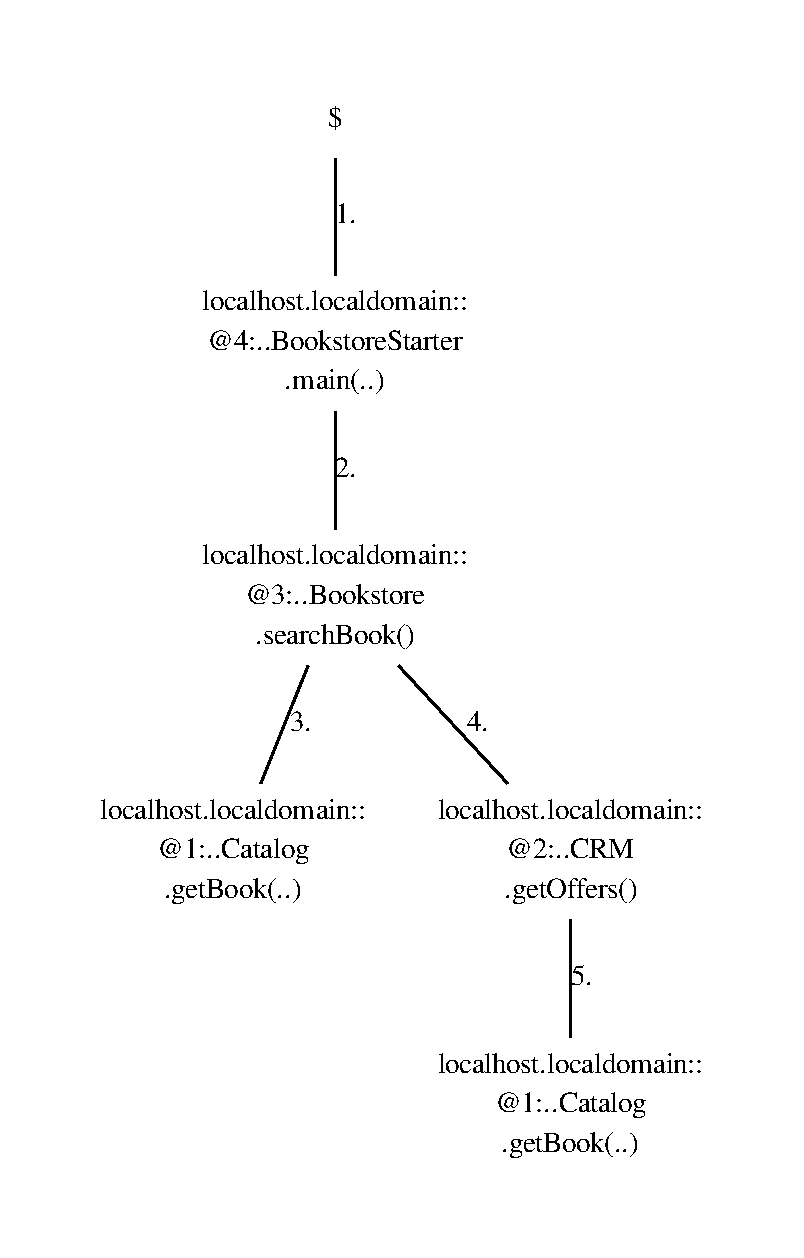
\includegraphics[height=0.4\textheight]{images/callTree}
%   }%
%   \subfigure[]{\label{fig:traceAnalysis:allocSeqDiagr}%
%   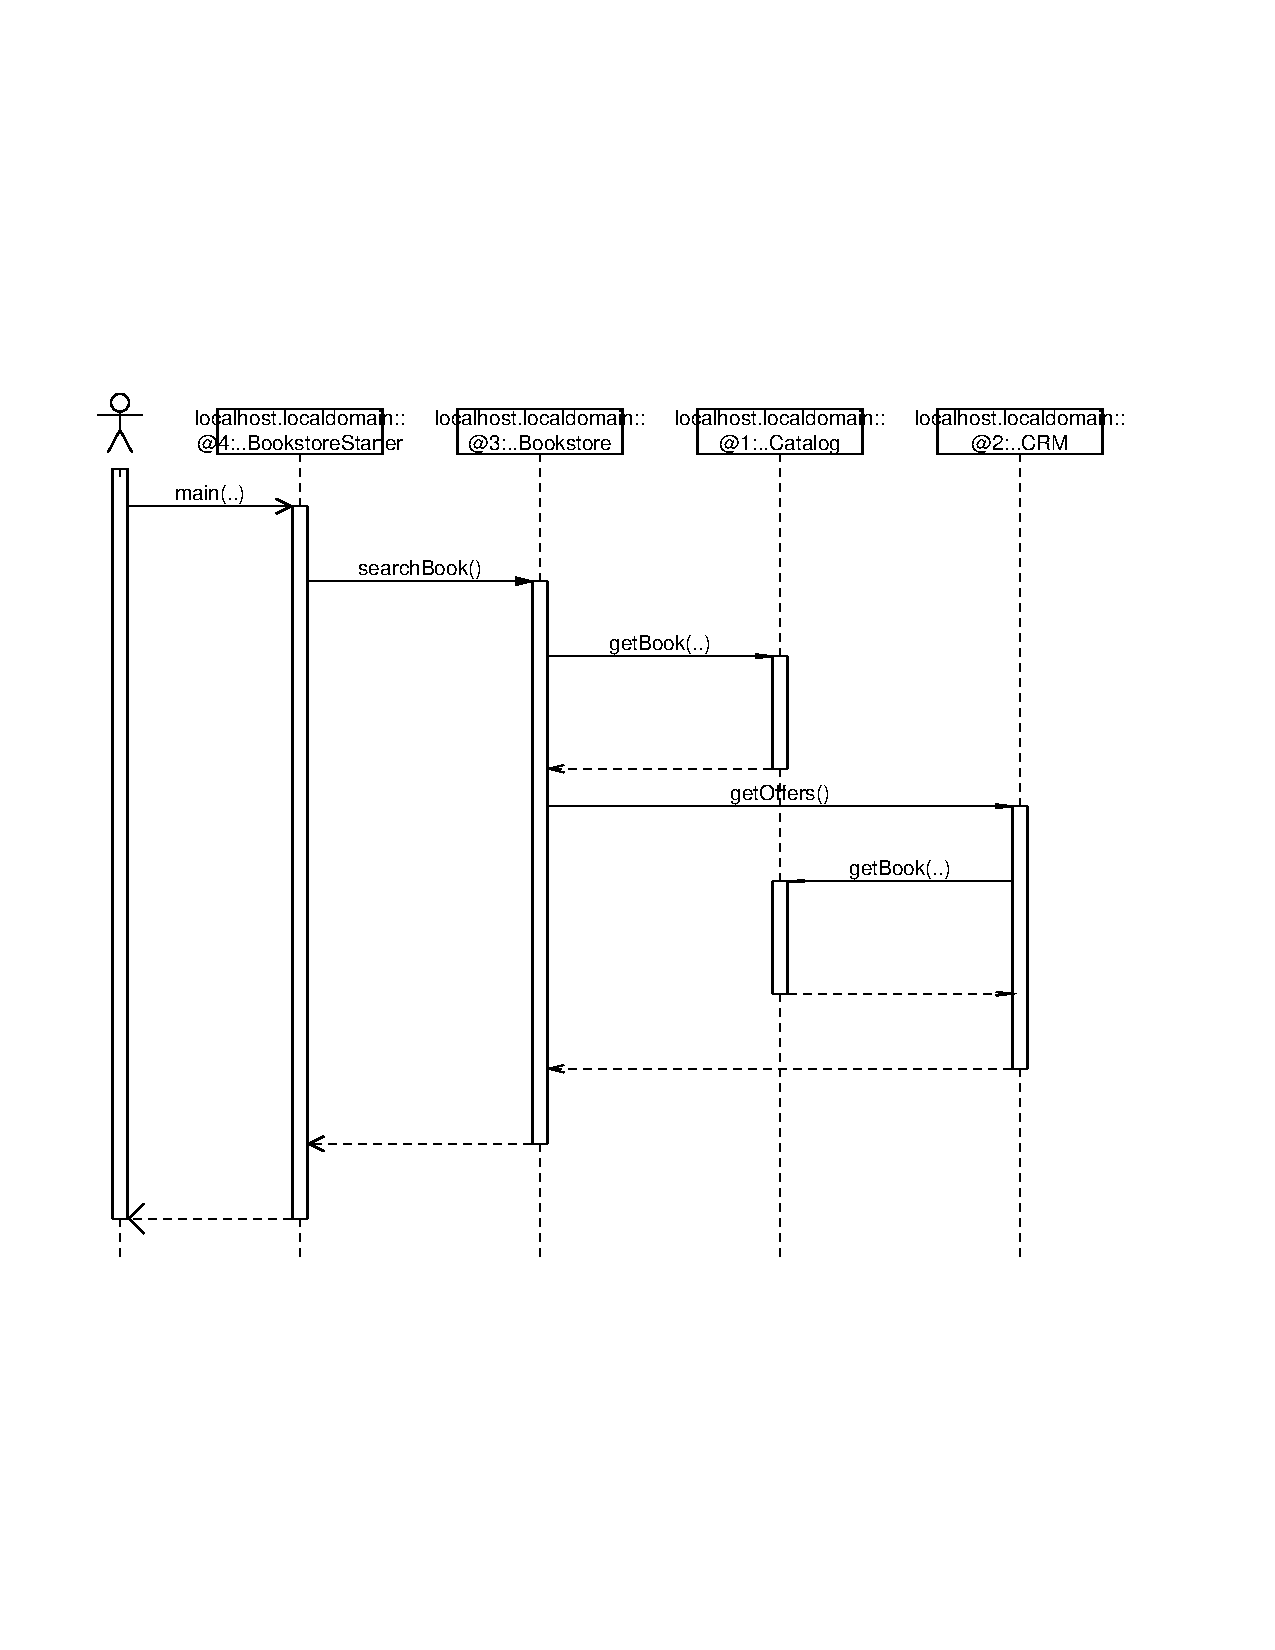
\includegraphics[height=0.4\textheight]{images/allocationSequenceDiagram}
%   }%
%
%   \caption{Call Tree~\subref{fig:traceAnalysis:callTree} and Allocation Sequence Diagram~\subref{fig:traceAnalysis:allocSeqDiagr}}
% \end{figure}

\NOTIFYBOX{The scripts \file{dotPic-fileConverter.sh} and \file{dotPic-fileConverter.bat} %
convert all \file{.pic} and \file{.dot} in a specified directory. %
See Appendix~\ref{appendix:wrapperScripts:dotPicFileConverter} for details.}

\vspace{5mm}

Examples of all available visualization are presented in the following %
Section~\ref{sec:traceAnalysisExamples}.

\pagebreak

\section{Example \KiekerTraceAnalysis{} Outputs}\label{sec:traceAnalysisExamples}
\newcommand{\OPT}[1]{\texttt{#1}}
\newcommand{\OPTprintValidExecutionTraces}{-\,-print-Execution-Traces}
\newcommand{\OPTprintInvalidExecutionTraces}{-\,-print-invalid-Execution-Traces}
\newcommand{\OPTprintMessageTraces}{-\,-print-Message-Traces}
\newcommand{\OPTprintDeploymentEquivalenceClasses}{-\,-print-Deployment-Equivalence-Classes}
\newcommand{\OPTprintAssemblyEquivalenceClasses}{-\,-print-Assembly-Equivalence-Classes}
\newcommand{\OPTplotDeploymentSequenceDiagrams}{-\,-plot-Deployment-Sequence-Diagrams}
\newcommand{\OPTplotAssemblySequenceDiagrams}{-\,-plot-Assembly-Sequence-Diagrams}
\newcommand{\OPTplotCallTrees}{-\,-plot-Call-Trees}
\newcommand{\OPTplotAggregatedDeploymentCallTree}{-\,-plot-Aggregated-Deployment-Call-Tree}
\newcommand{\OPTplotAggregatedAssemblyCallTree}{-\,-plot-Aggregated-Assembly-Call-Tree}

\newcommand{\OPTplotContainerDependencyGraph}{-\,-plot-Container-Dependency-Graph}
\newcommand{\OPTplotDeploymentComponentDependencyGraph}{-\,-plot-Deployment-Component-Dependency-Graph}
\newcommand{\OPTplotAssemblyComponentDependencyGraph}{-\,-plot-Assembly-Component-Dependency-Graph}
\newcommand{\OPTplotDeploymentOperationDependencyGraph}{-\,-plot-Deployment-Operation-Dependency-Graph}
\newcommand{\OPTplotAssemblyOperationDependencyGraph}{-\,-plot-Assembly-Operation-Dependency-Graph}

The examples presented in this section were generated based on the %
monitoring data which can be found in the directory %
\dir{\distributedTestdataDirDistro/}. It consists of 1635 traces %
of the Bookstore application with AspectJ-based instrumentation, %
as described in Section~\ref{sec:traceAnalysis:instr:AspectJ}. %
In order to illustrate the visualization of distributed traces, %
the hostname of the \class{Catalog}'s method \method{getBook} was %
probabilistically changed to a second hostname. %
For a more detailed description of the underlying formalisms, %
we refer to our technical report~\cite{vanHoornRohrHasselbringWallerEhlersFreyKieselhorst2009TRContinuousMonitoringOfSoftwareServicesDesignAndApplicationOfTheKiekerFramework}. %
The output can be found in the directory %
\dir{\distributedTestdataDirDistro-example-plots/}.

\subsection{Textual Trace and Equivalence Class Representations}

\subsubsection{Execution Traces}\label{sec:example:executionTraces}%

Textual execution trace representations of valid/invalid traces are written to %
an output file using the command-line options \OPT{\OPTprintValidExecutionTraces} and %
\OPT{\OPTprintInvalidExecutionTraces}. %
Listing~\ref{lst:appendix:traceAnalysisExample:executionTraces} %
shows the execution trace representation for the valid trace \ldots6129.

\setTextListing
\lstinputlisting[firstline=1,lastline=5,escapechar={},%
caption=Textual output of trace 6488138950668976129's execution trace representation,%
label=lst:appendix:traceAnalysisExample:executionTraces]%
{../../examples/userguide/ch5--trace-monitoring-aspectj/testdata/kieker-20100830-082225522-UTC-example-plots/executionTraces.txt} % macros don't work here ...

\subsubsection{Message Traces}\label{sec:example:messageTraces}%

Textual message trace representations of valid traces are written to an output %
file using the command-line option \OPT{\OPTprintMessageTraces}. %
Listing~\ref{lst:appendix:traceAnalysisExample:messageTraces} %
shows the message trace representation for the valid trace \ldots6129.

\setTextListing
\lstinputlisting[firstline=1,lastline=9,escapechar={},%
caption=Textual output of trace 6488138950668976129's message trace representation,%
label=lst:appendix:traceAnalysisExample:messageTraces]%
{../../examples/userguide/ch5--trace-monitoring-aspectj/testdata/kieker-20100830-082225522-UTC-example-plots/messageTraces.txt}

\subsubsection{Trace Equivalence Classes}\label{sec:example:traceEquivClasses}%

Deployment/assembly-level trace equivalence classes are computed and written %
to output files using the command-line options \OPT{\OPTprintDeploymentEquivalenceClasses} %
and \OPT{\OPTprintAssemblyEquivalenceClasses}. %
Listings~\ref{lst:appendix:traceAnalysisExample:traceDeploymentEquivClasses} and %
\ref{lst:appendix:traceAnalysisExample:traceAssemblyEquivClasses} show the %
output generated for the monitoring data used in this section. %

\setTextListing
\lstinputlisting[caption=Textual output of information on the \textit{deployment-level} trace equivalence classes,%
label=lst:appendix:traceAnalysisExample:traceDeploymentEquivClasses]
{../../examples/userguide/ch5--trace-monitoring-aspectj/testdata/kieker-20100830-082225522-UTC-example-plots/traceDeploymentEquivClasses.txt}

\setTextListing
\lstinputlisting[caption=Textual output of information on the \textit{assembly-level} trace equivalence class,%
label=lst:appendix:traceAnalysisExample:traceAssemblyEquivClasses]%
{../../examples/userguide/ch5--trace-monitoring-aspectj/testdata/kieker-20100830-082225522-UTC-example-plots/traceAssemblyEquivClasses.txt}

\pagebreak

\subsection{Sequence Diagrams}\label{sec:example:seqDiagrams}%

\subsubsection{Deployment-Level Sequence Diagrams}\label{sec:example:deploymentSeqDiagrams}%

Deployment-level sequence diagrams are generated using the command-line option \OPT{\OPTplotDeploymentSequenceDiagrams}. %
Figures~\ref{fig:appendix:traceAnalysisExample:SeqDiagrsDepl6129}--\ref{fig:appendix:traceAnalysisExample:SeqDiagrsDepl6141} %
show these sequence diagrams for each deployment-level %
trace equivalence representative (Section~\ref{sec:example:traceEquivClasses}).

\begin{figure}[h]\centering
\subfigure[Trace \ldots{}6129]{\label{fig:appendix:traceAnalysisExample:SeqDiagrsDepl6129}%
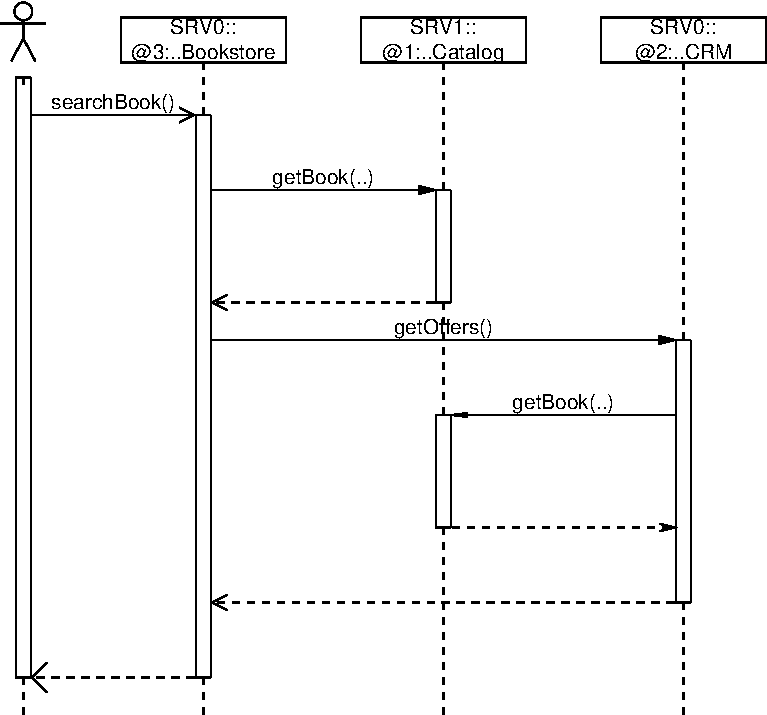
\includegraphics[scale=0.39]{../../examples/userguide/ch5--trace-monitoring-aspectj/testdata/kieker-20100830-082225522-UTC-example-plots/deploymentSequenceDiagram-6488138950668976129-crop}
}
\subfigure[Trace \ldots{}6130]{\label{fig:appendix:traceAnalysisExample:SeqDiagrsDepl6130}%
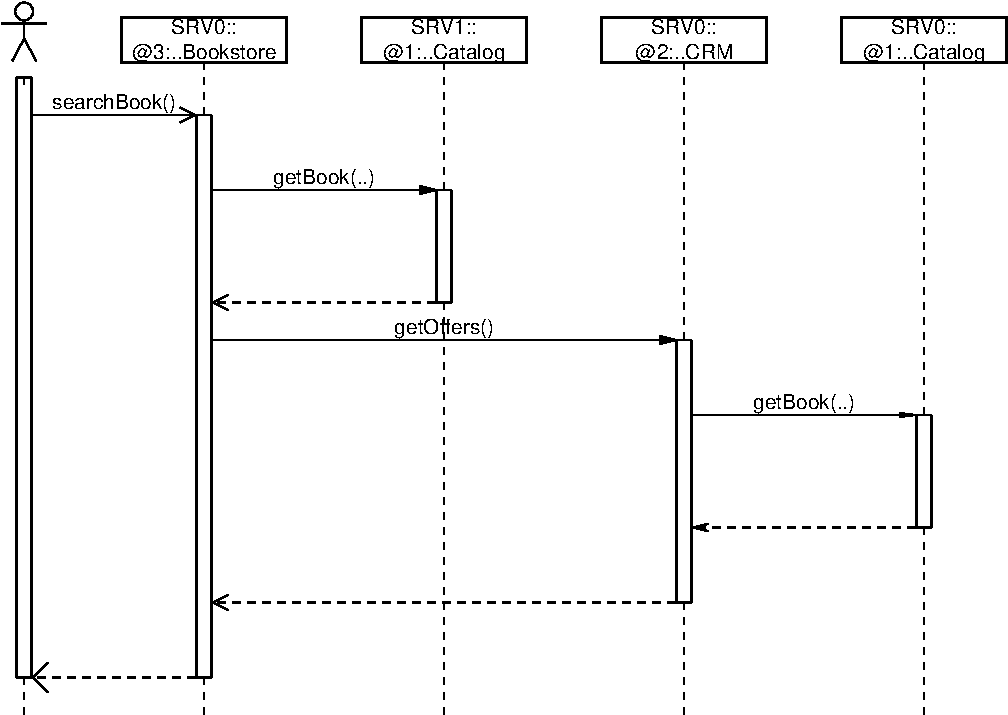
\includegraphics[scale=0.39]{../../examples/userguide/ch5--trace-monitoring-aspectj/testdata/kieker-20100830-082225522-UTC-example-plots/deploymentSequenceDiagram-6488138950668976130-crop}
}
\subfigure[Trace \ldots{}6131]{\label{fig:appendix:traceAnalysisExample:SeqDiagrsDepl6131}%
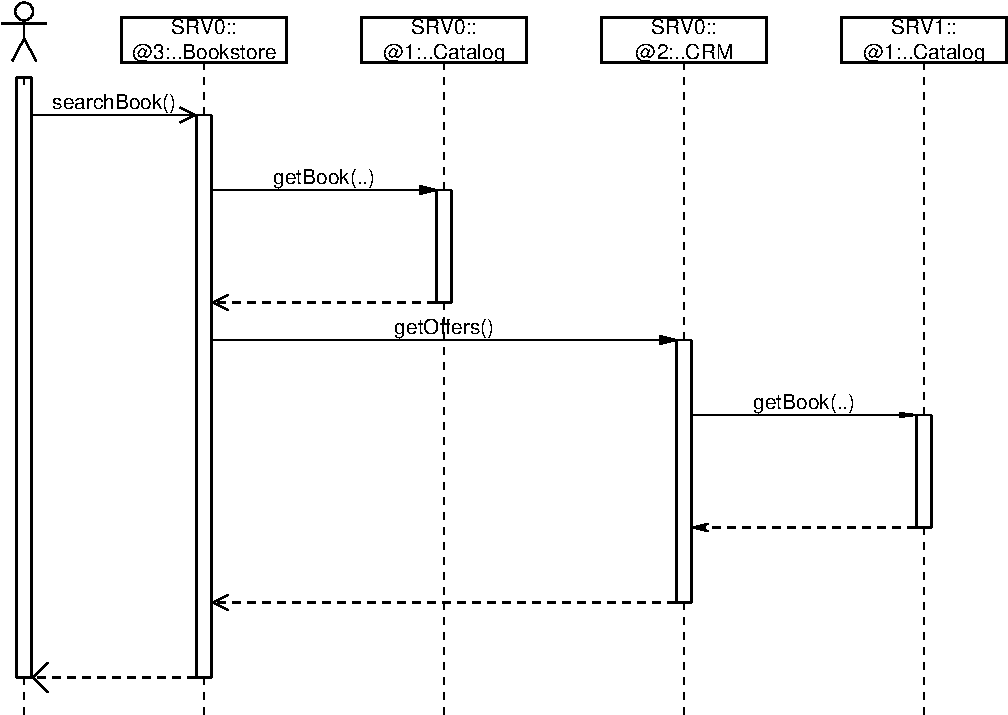
\includegraphics[scale=0.39]{../../examples/userguide/ch5--trace-monitoring-aspectj/testdata/kieker-20100830-082225522-UTC-example-plots/deploymentSequenceDiagram-6488138950668976131-crop}
}
\subfigure[Trace \ldots{}6141]{\label{fig:appendix:traceAnalysisExample:SeqDiagrsDepl6141}%
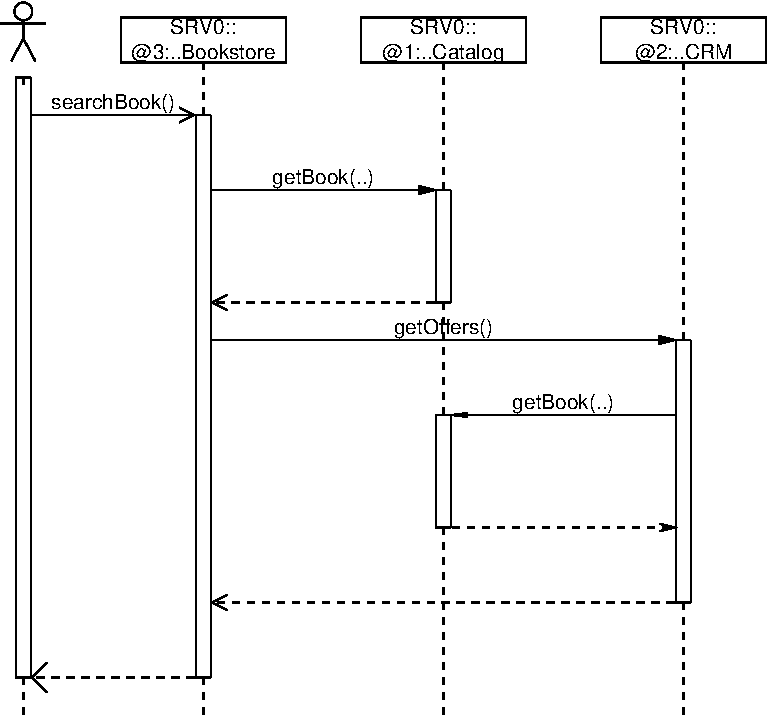
\includegraphics[scale=0.39]{../../examples/userguide/ch5--trace-monitoring-aspectj/testdata/kieker-20100830-082225522-UTC-example-plots/deploymentSequenceDiagram-6488138950668976141-crop}
}
\caption{\textit{Deployment-level} sequence diagrams of the trace %
equivalence class representatives (Listing~\ref{lst:appendix:traceAnalysisExample:traceAssemblyEquivClasses})}
\label{fig:appendix:traceAnalysisExample:SeqDiagrsDepl}
\end{figure}

% \enlargethispage{2cm}
\pagebreak

\subsubsection{Assembly-Level Sequence Diagrams}\label{sec:example:assemblySeqDiagrams}%

Assembly-level sequence diagrams are generated using the command-line option \OPT{\OPTplotAssemblySequenceDiagrams}. %
Figure~\ref{fig:appendix:traceAnalysisExample:SeqDiagrDepl6129} %
shows the sequence diagram for the assembly-level trace equivalence representative %
(Section~\ref{sec:example:traceEquivClasses}).

\begin{figure}[h]\centering
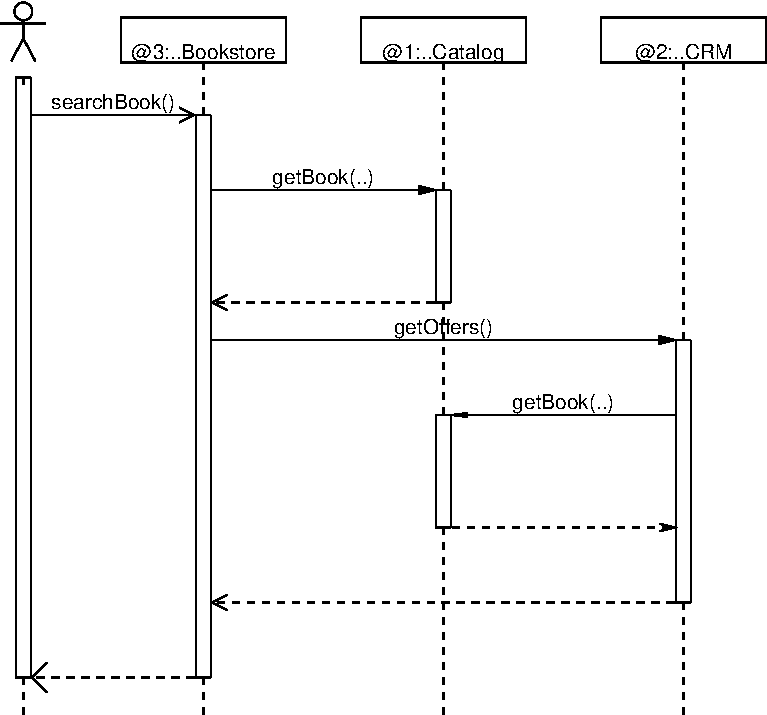
\includegraphics[scale=0.39]{../../examples/userguide/ch5--trace-monitoring-aspectj/testdata/kieker-20100830-082225522-UTC-example-plots/assemblySequenceDiagram-6488138950668976129-crop}
\caption{\textit{Assembly-level} sequence diagram of trace \ldots{}6129}
\label{fig:appendix:traceAnalysisExample:SeqDiagrDepl6129}
\end{figure}

% \pagebreak

\subsection{Call Trees}\label{sec:example:callTrees}%

\subsubsection{Trace Call Trees}\label{sec:example:traceCallTrees}%

\enlargethispage{1.2cm}

Trace call trees are generated using the command-line option \OPT{\OPTplotCallTrees}. %
Figures~\ref{fig:appendix:traceAnalysisExample:TraceCallTrees6129}--\ref{fig:appendix:traceAnalysisExample:TraceCallTrees6141} %
show these call trees for each deployment-level %
trace equivalence representative (Section~\ref{sec:example:traceEquivClasses}).

\begin{figure}[h]\centering
\subfigure[Trace \ldots{}6129]{\label{fig:appendix:traceAnalysisExample:TraceCallTrees6129}%
\ \ 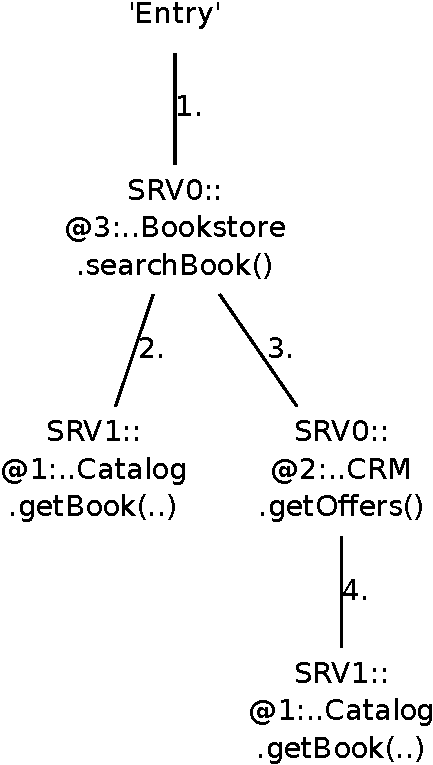
\includegraphics[scale=0.4]{../../examples/userguide/ch5--trace-monitoring-aspectj/testdata/kieker-20100830-082225522-UTC-example-plots/callTree-6488138950668976129-crop}\ \ 
}
\subfigure[Trace \ldots{}6130]{\label{fig:appendix:traceAnalysisExample:TraceCallTrees6130}%
\ \ 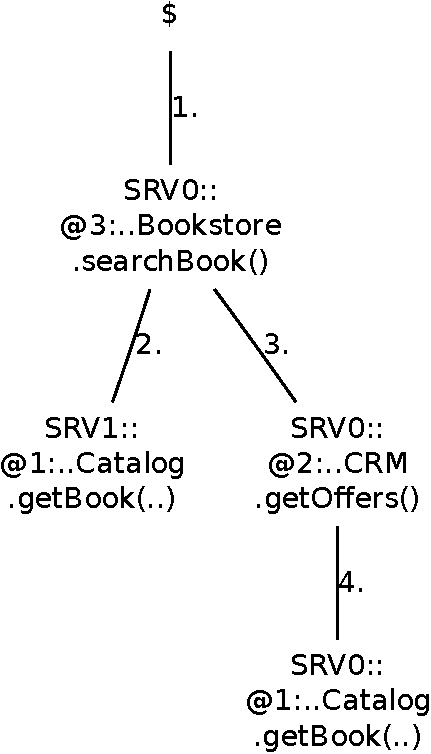
\includegraphics[scale=0.4]{../../examples/userguide/ch5--trace-monitoring-aspectj/testdata/kieker-20100830-082225522-UTC-example-plots/callTree-6488138950668976130-crop}\ \ 
}
\subfigure[Trace \ldots{}6131]{\label{fig:appendix:traceAnalysisExample:TraceCallTrees6131}%
\ \ 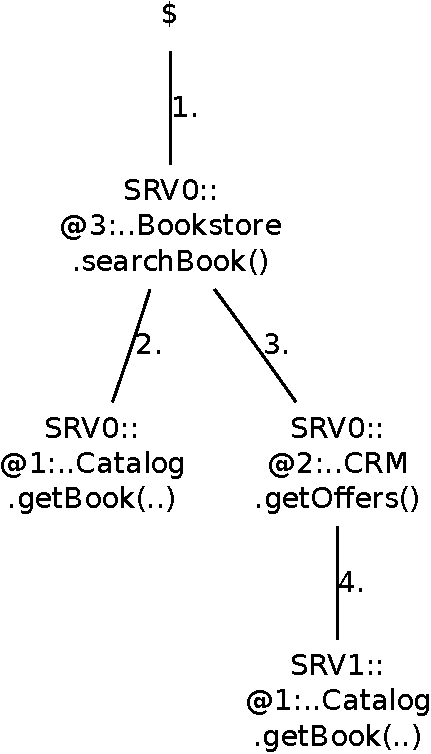
\includegraphics[scale=0.4]{../../examples/userguide/ch5--trace-monitoring-aspectj/testdata/kieker-20100830-082225522-UTC-example-plots/callTree-6488138950668976131-crop}\ \ 
}
\subfigure[Trace \ldots{}6141]{\label{fig:appendix:traceAnalysisExample:TraceCallTrees6141}%
\ \ 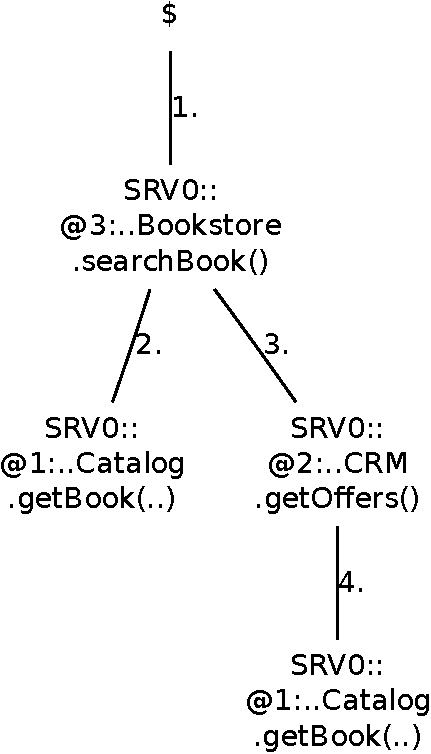
\includegraphics[scale=0.4]{../../examples/userguide/ch5--trace-monitoring-aspectj/testdata/kieker-20100830-082225522-UTC-example-plots/callTree-6488138950668976141-crop}\ \ 
}
\caption{Calls trees of the trace %
equivalence class representatives (Listing~\ref{lst:appendix:traceAnalysisExample:traceAssemblyEquivClasses})}
\label{fig:appendix:traceAnalysisExample:TraceCallTrees}
\end{figure}

% \newpage

\subsubsection{Aggregated Call Trees}\label{sec:example:aggregatedCallTrees}%

Aggregated deployment/assembly-level call trees are generated using the command-line options %
\OPT{\OPTplotAggregatedDeploymentCallTree} and \OPT{\OPTplotAggregatedAssemblyCallTree}. %
Figures~\ref{fig:appendix:traceAnalysisExample:AggregatedCallTreesDeployment} and \ref{fig:appendix:traceAnalysisExample:AggregatedCallTreesAssembly} %
show these aggregated call trees for the traces contained in the monitoring data %
used in this section. %

\begin{figure}[h]\centering
\subfigure[deployment-level]{\label{fig:appendix:traceAnalysisExample:AggregatedCallTreesDeployment}%
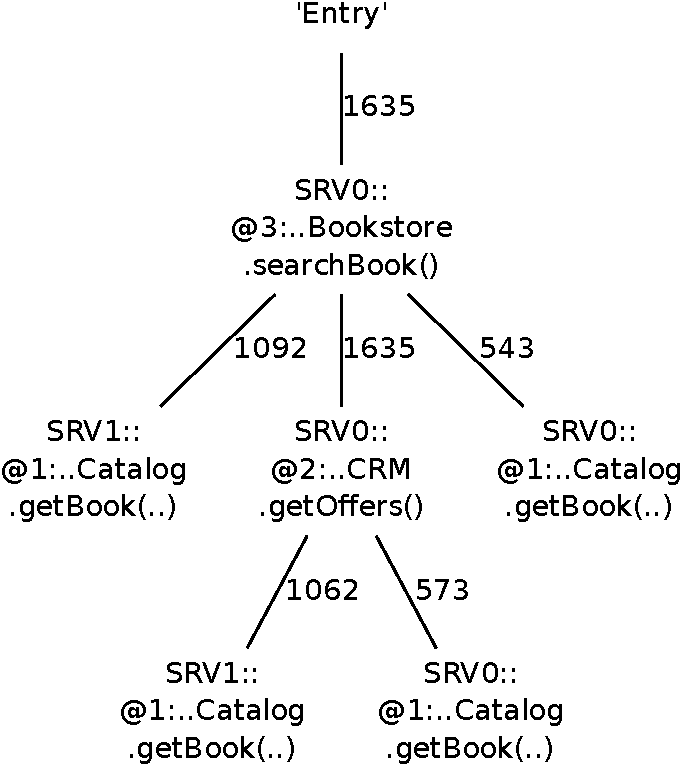
\includegraphics[scale=0.4]{../../examples/userguide/ch5--trace-monitoring-aspectj/testdata/kieker-20100830-082225522-UTC-example-plots/aggregatedDeploymentCallTree-crop}%
}
\subfigure[assembly-level]{\label{fig:appendix:traceAnalysisExample:AggregatedCallTreesAssembly}%
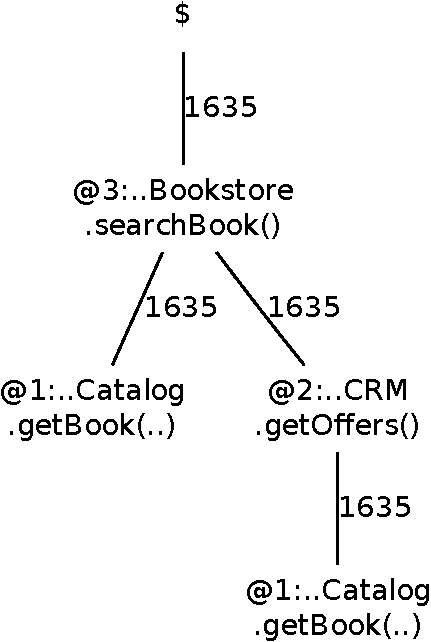
\includegraphics[scale=0.4]{../../examples/userguide/ch5--trace-monitoring-aspectj/testdata/kieker-20100830-082225522-UTC-example-plots/aggregatedAssemblyCallTree-crop}%
}
\caption{Aggregated call trees generated from the 1635~traces}
\label{fig:appendix:traceAnalysisExample:AggregatedCallTrees}
\end{figure}

\pagebreak

\subsection{Dependency Graphs}

\subsubsection{Container Dependency Graphs}

A container dependency graph is generated using the command-line option %
\OPT{\OPTplotContainerDependencyGraph}. %
Figure~\ref{fig:appendix:traceAnalysisExample:ContainerDepGraph} shows the %
container dependency graph for the monitoring data used in this section. 

\begin{figure}[h]\centering
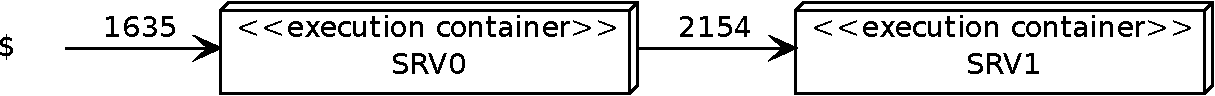
\includegraphics[scale=0.45]{../../examples/userguide/ch5--trace-monitoring-aspectj/testdata/kieker-20100830-082225522-UTC-example-plots/containerDependencyGraph-crop}
\caption{Container dependency graph}
\label{fig:appendix:traceAnalysisExample:ContainerDepGraph}
\end{figure}

\subsubsection{Component Dependency Graphs}

Deployment/assembly-level component dependency graphs are generated using the %
command-line options \OPT{\OPTplotDeploymentComponentDependencyGraph} and %
\OPT{\OPTplotAssemblyComponentDependencyGraph}. %
Figures~\ref{fig:appendix:traceAnalysisExample:ComponentDepGraphsDeployment} and %
\ref{fig:appendix:traceAnalysisExample:ComponentDepGraphsAssembly} show the %
component dependency graphs for the monitoring data used in this section. 

\begin{figure}[h]\centering
\subfigure[deployment-level]{\label{fig:appendix:traceAnalysisExample:ComponentDepGraphsDeployment}%
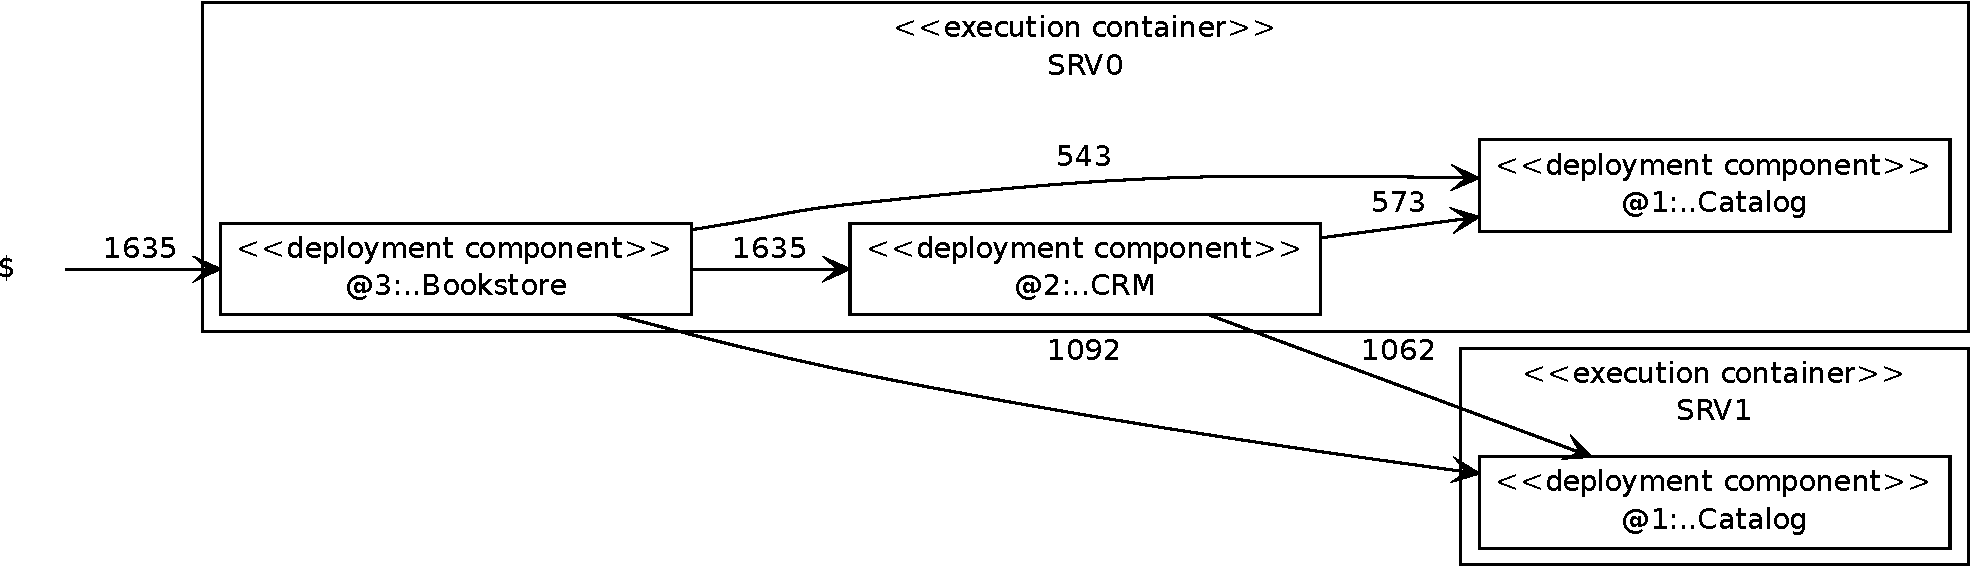
\includegraphics[scale=0.45]{../../examples/userguide/ch5--trace-monitoring-aspectj/testdata/kieker-20100830-082225522-UTC-example-plots/deploymentComponentDependencyGraph-crop}
}
\subfigure[assembly-level]{\label{fig:appendix:traceAnalysisExample:ComponentDepGraphsAssembly}%
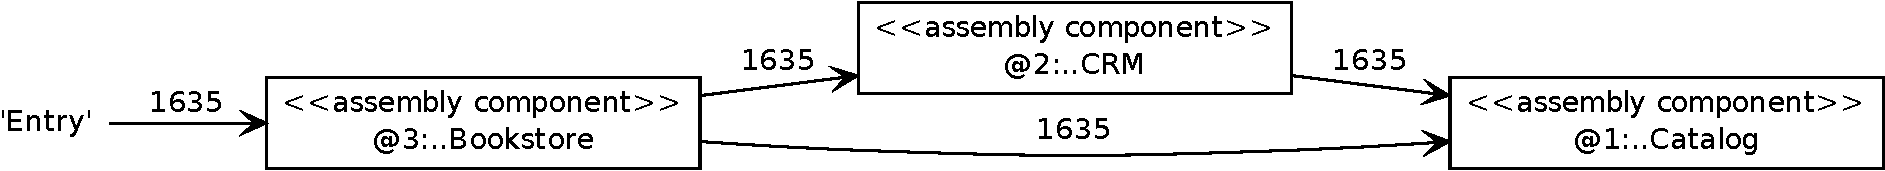
\includegraphics[scale=0.45]{../../examples/userguide/ch5--trace-monitoring-aspectj/testdata/kieker-20100830-082225522-UTC-example-plots/assemblyComponentDependencyGraph-crop}
}
\caption{Component dependency graphs}
\label{fig:appendix:traceAnalysisExample:ComponentDepGraphs}
\end{figure}

\pagebreak

\subsubsection{Operation Dependency Graphs}

Deployment/assembly-level operation dependency graphs are generated using the %
command-line options \OPT{\OPTplotDeploymentOperationDependencyGraph} and %
\OPT{\OPTplotAssemblyOperationDependencyGraph}. %
Figures~\ref{fig:appendix:traceAnalysisExample:OperationDepGraphsDeployment} and %
\ref{fig:appendix:traceAnalysisExample:OperationDepGraphsAssembly} show the %
operation dependency graphs for the monitoring data used in this section. 

\begin{figure}[ht]\centering
\subfigure[deployment-level]{\label{fig:appendix:traceAnalysisExample:OperationDepGraphsDeployment}%
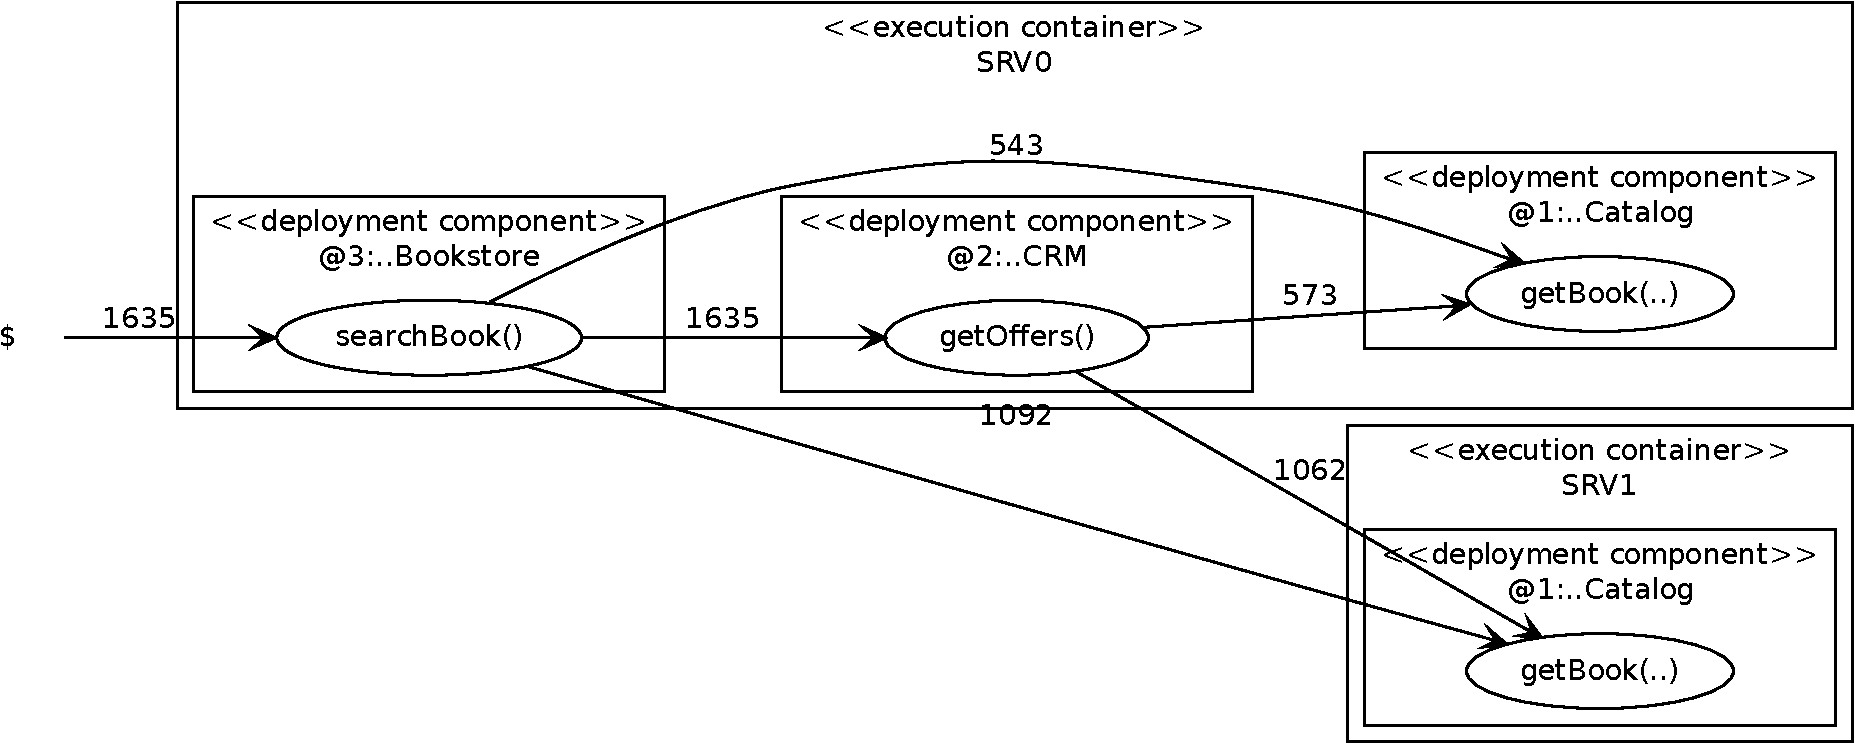
\includegraphics[scale=0.4]{../../examples/userguide/ch5--trace-monitoring-aspectj/testdata/kieker-20100830-082225522-UTC-example-plots/deploymentOperationDependencyGraph-crop}
}
\subfigure[assembly-level]{\label{fig:appendix:traceAnalysisExample:OperationDepGraphsAssembly}%
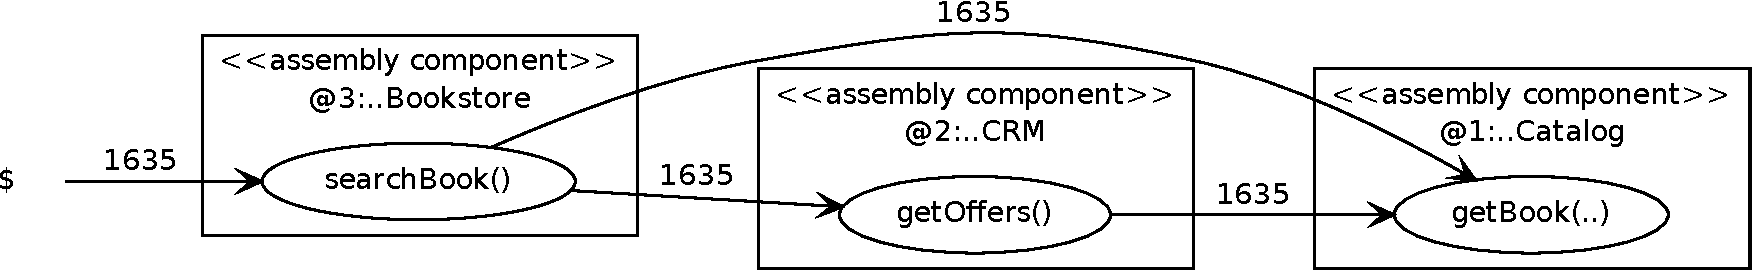
\includegraphics[scale=0.4]{../../examples/userguide/ch5--trace-monitoring-aspectj/testdata/kieker-20100830-082225522-UTC-example-plots/assemblyOperationDependencyGraph-crop}
}
\caption{Operation dependency graphs}
\label{fig:appendix:traceAnalysisExample:OperationDepGraphs}
\end{figure}

\pagebreak

\subsection{Response Times in Dependency Graphs}

The afore-mentioned dependency graphs can also be decorated by the response times, adding the minimum, the average, %
and the maximum response times of the components. The decoration will be generated with the additional command line %
parameter \OPT{responseTimes} behind the corresponding \OPT{plot-}command.  %
An exemplaric graph with response times is shown in Figure~\ref{fig:appendix:traceAnalysisExample:graphWithRespTimes}.

\begin{figure}[h]
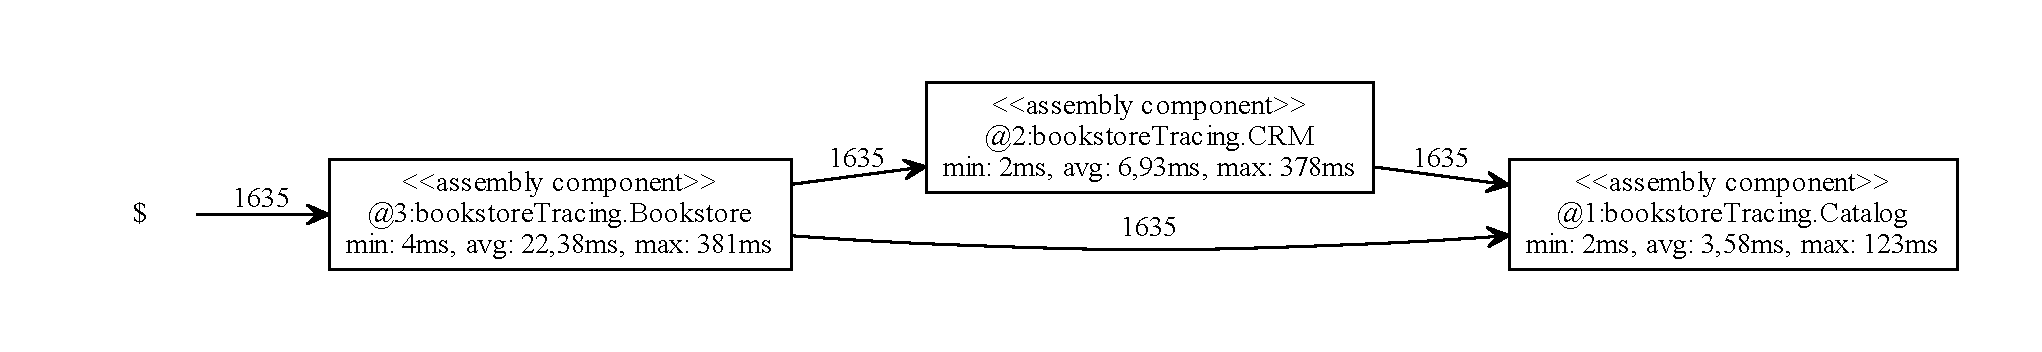
\includegraphics[scale=0.45]{images/assemblyComponentDependencyGraphWithResponseTimes}
\caption{Assembly component dependency graph with response times}
\label{fig:appendix:traceAnalysisExample:graphWithRespTimes}
\end{figure}
   

\pagebreak

\subsection{HTML Output of the System Model}

\KiekerTraceAnalysis{} writes an HTML representation of the system model reconstructed %
from the trace data to a file \file{system-entities.html}. %
Figure~\ref{fig:appendix:traceAnalysisExample:htmlSystemModel} shows a screenshot %
of this file rendered by a web browser.

\begin{figure}[h]\centering
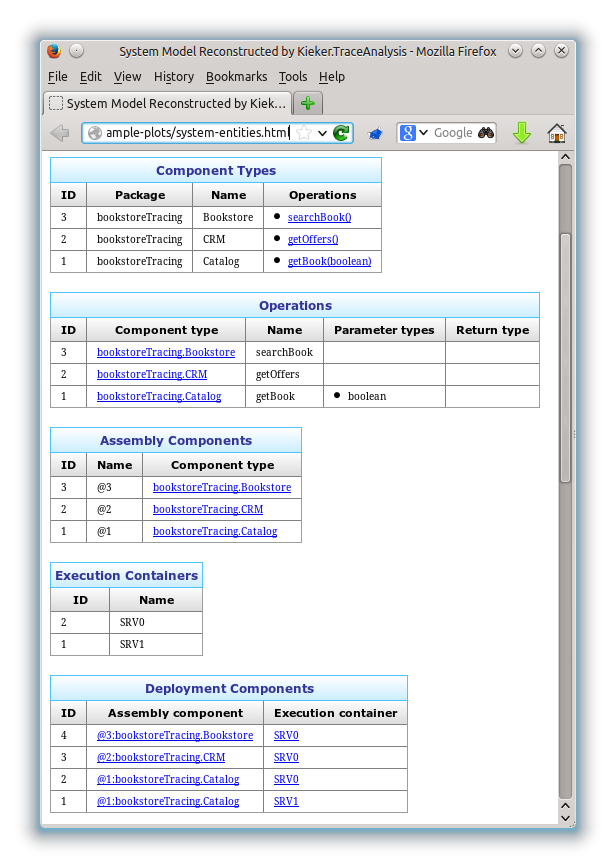
\includegraphics[width=0.7\textwidth]{images/system-entities-html-FFscrsh.png}
\caption{HTML output of the system model reconstructed from the traces}
\label{fig:appendix:traceAnalysisExample:htmlSystemModel}
\end{figure}

